\section{Implementation}

\subsection{Architecture}

{\sloppy\textit{qPCRtools} is written in C++17 and built on Qt6 \cite{qt}. The user
interface is rendered with web technologies---Bootstrap~5.3 for layout and
Apache ECharts \cite{echarts} for figures---inside a
\texttt{QWebEngineView}, and exchanges data with the native backend through
Qt~WebChannel. All numerical computation therefore stays in compiled code
while the presentation layer remains plain HTML, CSS and JavaScript. The
analytical core is a standalone static library, \texttt{qpcr\_core}, that
depends only on Qt~Core (plus optional Eigen and GSL) and is independent of
the GUI, so it is exercised directly by the unit tests and by the
command-line validation driver. Figure~\ref{fig:overview} shows the
interface at the end of a complete analysis.\par}

\begin{figure}[tbp]
\centering
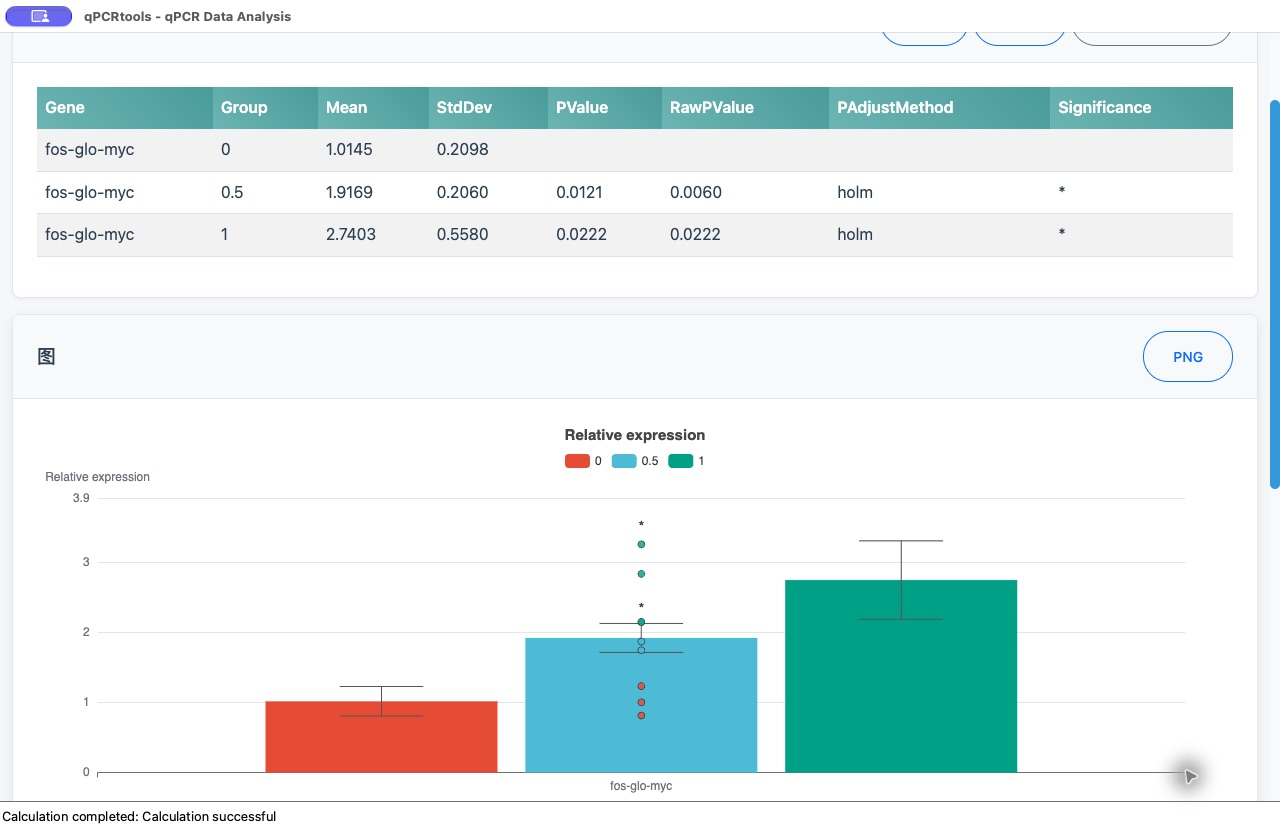
\includegraphics[width=0.85\linewidth]{figures/fig1_results_page_en_v4_20261029.png}
\caption{The \textit{qPCRtools} desktop interface (screen capture of
version~1.3.0). The upper panel is the summary table from the bundled
example---the target gene \textit{fos-glo-myc} normalised to
\textit{Beta Actin},
three dose groups with three biological replicates each---analysed by the
$\Delta\Delta C_t$ method with Welch tests against the control. It reports
the mean, standard deviation, Holm-adjusted and raw $P$ values, adjustment
method and significance symbol. The lower panel redraws the group means with
standard-deviation error bars, individual biological replicates and
Holm-adjusted symbols; the error bars are not repeated as a legend entry.
The interface is bilingual (Chinese/English); the English language is
shown here.}
\label{fig:overview}
\end{figure}

\subsection{Quantification algorithms}

The core reimplements the methods of the R package. Amplification efficiency
is obtained by ordinary least squares of $C_q$ on
$\log_{d}(\text{concentration})$, i.e.\ the number of $d$-fold dilution
steps ($d$ = dilution factor, 4 in the bundled example), yielding slope $s$,
intercept, $R^2$ and a regression $P$-value; efficiency is
\begin{equation}
E = d^{-1/s} - 1,
\end{equation}
with $s$ expressed per $\log_d$ unit (equivalently, per dilution step).
Relative expression is computed by the
$\Delta C_t$ and $\Delta\Delta C_t$ methods \cite{livak2001analysis},
\begin{equation}
\mathrm{RE} = 2^{-\big[(C_{q,\mathrm{target}}-C_{q,\mathrm{ref}})_{\mathrm{treated}}
- \overline{(C_{q,\mathrm{target}}-C_{q,\mathrm{ref}})}_{\mathrm{control}}\big]},
\end{equation}
where the first term is sample-level and the overbar is the mean $\Delta C_t$
across control biological replicates. Relative expression is also computed
by an efficiency-based (RqPCR) method \cite{rancurel2019satqpcr} in which
per-sample quantities are $E^{\,C_{q,\min}-C_q}$, normalized by the geometric
mean of one or more reference genes \cite{pfaffl2001new}. In this method
$C_{q,\min}$ is obtained separately within each biological replicate across
the treatments, so the calculation is a within-block comparison rather than a
general unpaired design. Efficiencies are supplied per gene in the design
table (or estimated by the built-in standard-curve module).

\subsection{Statistical analysis}

{\sloppy Groups are compared on the linear relative-expression scale, which is
the scale on which values are reported and plotted. Because the linear and
$\Delta C_t$ scales can give different $P$ values for the same data, the
$\Delta C_t$-scale comparison is reported as a sensitivity analysis in
Supplementary Table~S2. The core
library implements Welch and Student two-sample $t$-tests, the paired
$t$-test, Wilcoxon rank-sum and signed-rank tests, one-way ANOVA with Tukey
HSD letters, Cohen's $d$, IQR-based outlier removal and automatic
reference-gene selection by geNorm \cite{vandesompele2002accurate}; the
interface exposes the Welch $t$-test, the rank-sum test and ANOVA with Tukey
HSD, while the paired tests are covered by the test suite but not yet offered
in the interface. When several groups are compared with the same control,
Welch and rank-sum $P$ values are adjusted by Holm's method within each gene,
and the unadjusted value is retained in the exported table. ANOVA uses Tukey
HSD. Correction is not applied across genes, which we state as a
limitation.\par}

\subsection{Software engineering and scope}

Results are shown as tables that can be exported as CSV or Excel, with Tukey
letters in the table. The application renders the figures in the interface:
group means with standard-deviation error bars and significance labels, and
the fitted standard curves over the measured dilution series, both exportable
as PNG images. Each analysis can also be exported as a plain-text
\emph{analysis record} listing the input files and their row counts, the
reference gene(s), the control group, the statistical test, the
outlier-removal setting, the software version and a timestamp, so that a
reader can re-run the analysis without inspecting the session. Quality
control is reported as warnings rather than decisions: wells with $C_q$ above
a configurable limit (default 35), samples whose technical replicates differ
by more than a configurable standard deviation (default 0.5~$C_q$), and
primers with efficiency outside 90--110\% are listed on the results page and
repeated in the analysis record, while no data are removed automatically.
MIQE~2.0 requires these quantities to be reported rather than to satisfy fixed
cut-offs \cite{bustin2025miqe2}, so the defaults are meant to be adapted to
the instrument and assay. \textit{qPCRtools} is managed with CMake and ships
with unit tests; the interface is bilingual and reads CSV/TXT input, and Excel
(\texttt{.xlsx}) workbooks when built with the optional OpenXLSX component
(the released binaries read CSV/TXT). It is distributed as a single
self-contained executable for Windows and macOS, requiring no R, Python or
runtime installation. The macOS binary is built for Apple Silicon, requires
macOS~12 or newer, and is ad-hoc signed but not notarized. Linux builds are
supported by the source and build scripts but are not part of the released
binary set. Two R
functions are not yet ported---the standard-curve
slope--intercept quantification (\texttt{CalExpCurve}) and the
reverse-transcription reagent volume calculation (\texttt{CalRTable})---and
are planned for a future release.
